\documentclass[11pt]{article}

% set these commands
\newcommand{\course}{CSCI 534}
\newcommand{\proj}{Homework 01}
\newcommand{\dueDate}{1-28-2021}
\newcommand{\name}{Nathan Stouffer}

\usepackage{../macros}

\newcommand{\pareto}[1]{\rm{Pareto}(#1)}
\newcommand{\conv}[1]{\rm{conv}(#1)}

\begin{document}

{ ~\\
    \course \\
    \proj \\
    Due \dueDate \\
    \name
}

\section*{Problem 1 (10 points)}

Let $P = \{ p_1, \ldots, p_n \}$ and $P' = \{ p_1', \ldots, p_n' \}$ be the
vertex sets of two upper hulls in the plane.  Each set is presented as a
sequence of points sorted from left to right.  Let $p_i = (x_i, y_i)$ and $p_j'
= (x_j', y_j')$ denote the point coordinates.  We assume that $P$ lies entirely
to the left of $P'$, meaning that there exists a value $z$ such that for all
$i$ and $j$, $x_i < z < x_j'$.

\begin{figure}[h]
    \centering
    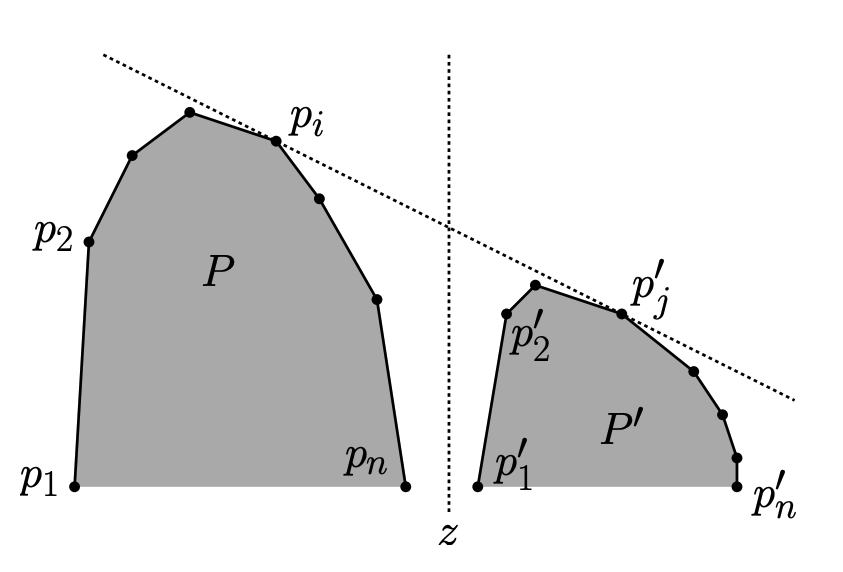
\includegraphics[width=0.5\textwidth]{tangents}
    \caption{Problem 1: Computing the upper tangent of two hulls}
\end{figure}

Present an $O(\log n)$-time algorithm which, given $P$ and $P'$, compute the two
points $p_i \in P$ and $p_j' \in P'$ such that their common support line passes
through these two points.

Briefly justify your algorithm's correctness and drive its running time.  ({\bf
Hint:} The correctness proof involves a case analysis.  Please be careful, a
poorly drawn figure may lead to an incorrect hypothesis.)

\section*{Problem 2 (20 points)}

Consider a set $P = \{p_1, \ldots, p_n \}$ of points in the plane, where $p_i =
(x_i, y_i)$. A \emph{Pareto set} for $P$, denoted $\pareto{P}$, (named after
the Italian engineer and economist Vilfredo Pareto), is a subset of points
$p_i$ such that there is no $p_j \in P (j \neq i)$ such that $x_j \geq x_i$ and
$y_j \geq y_i$.  That is, each point of $\pareto{P}$ has the property that
there is no point of $P$ that is both to the right and above it.

\begin{figure}[h]
    \centering
    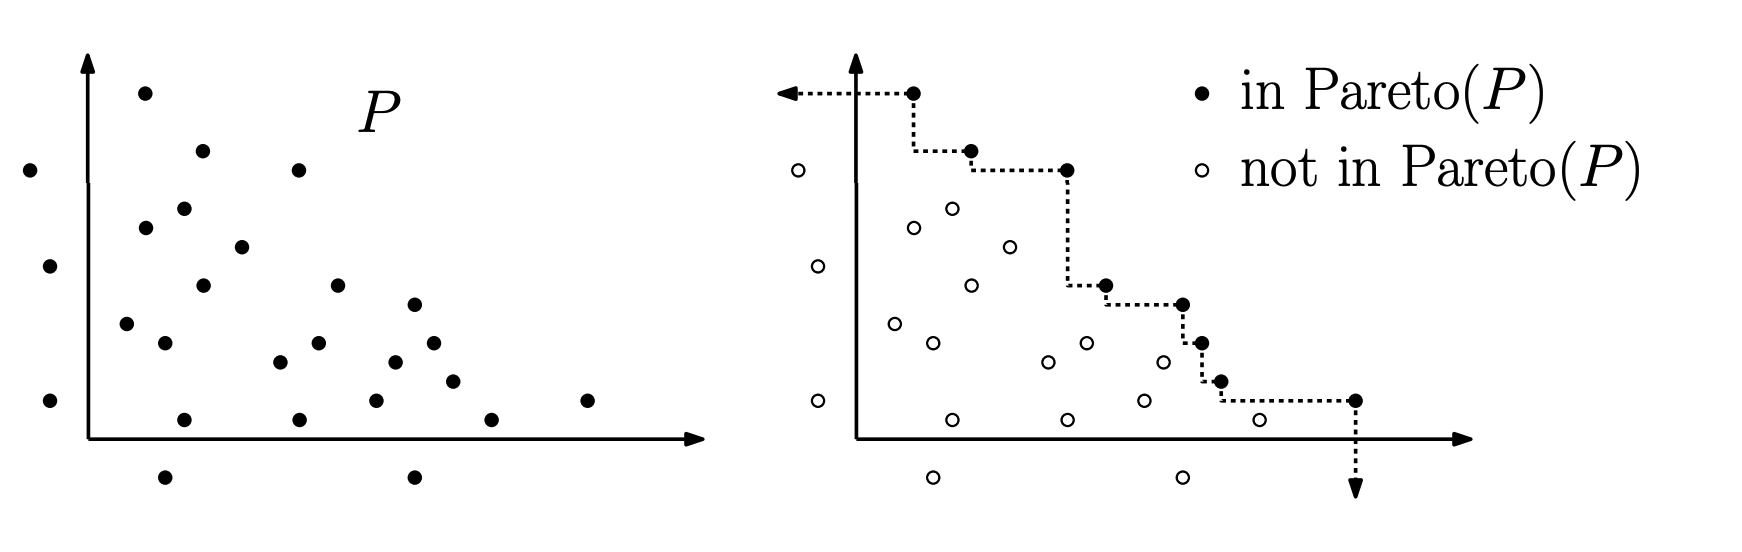
\includegraphics[width=0.75\textwidth]{pareto}
    \caption{Problem 2: Pareto set}
\end{figure}

Pareto sets and convex hulls in the plane are similar in many respects.  In
this problem we will explore some of these connections.

\begin{enumerate}

\item (5 points) A point $p$ lies on the convex hull of a set $P$ if and only if there is
a line passing though $p$ such that all the points of $P$ lie on one side of
this line.  Provide an analogous assertion for the points of $\pareto{P}$ in
terms of a different shape.

\answer
Our goal is to provide some geometric condition that conveys whether a point is a member of $\pareto{P}$.
For the convex hull, a point $p$ was on the convex hull of a set $P$ if and only if there is a line passing through $p$ such that all points of $P$ lie on one side of the line.
This is equivalent to requiring that there exists a half plane (with $p$ on the line defining the half plane) such that all points in $P$ are on one side of the half plane.
For the $\pareto{P}$, we have a similar requirement with a ``quarter'' plane.
Consider a plane with $p$ at the origin and axes in the regular directions.
Then $p$ is in $\pareto{P}$ if and only if no points in $P$ are inside (or on the border) of the first quadrant of the plane centered at $p$.
If $p$ is in the $\pareto{P}$ the no point $p'$ has both $x' \geq x$ and $y' \geq y$ so $p$ so no values can be in the first quadrant.
Proving the converse (via contrapositive), if some point $p'$ is inside the first quadrant, then both $x' \geq x$ and $y' \geq y$ so $p$ cannot be in $\pareto{P}$.

\item (5 points) Devise an analogue of Graham's convex-hull algorithm for computing
\pareto{P} in $O(n \log n)$ time.  Briefly justify your algorithm's correctness
and derive its running time.  (You do not need to explain the algorithm ``from
scratch'', that is, you can explain with modifications would be made to Grahm's
algorithm.)

\answer
First we give a quick description of the algorithm (relative to Graham's Scan).
Instead of sorting the points in increasing order (like Graham's Scan), sort them in increasing order according to their $x$ coordinate: $P = \{ p_1, p_2, ..., p_n \}$ where $i < j$ implies $x_i > x_j$.
Then push $p_1$ on to the stack $S$.
Then for $i$ from $2$ to $n$, if $y_i \geq S[top]_y$ (where $S[top]_y$ is the $y$ coordinate of the point $S[top]$) then push $p_i$ to the stack.

Now let's analyze the runtime.
The sorting step takes $O(n \log n)$ time and then we do a scan through all the data points in $O(n)$ time.
So the total run time for this algorithm is $O(n \log n) + O(n) = O(n \log (n) + n) = O(n \log n)$.

Now we give a discussion of correctnes.
Post sorting, we know $p_1 \in \pareto{P}$ by the following line of reasoning.
The definition of $\pareto{P}$ is a subset of points $p_i$ such that there is no $p_j \in P (j \neq i)$ such that $x_j \geq x_i$ and $y_j \geq y_i$.
This is equivalent to a subset of points $p_i$ such that $\forall p_j \in P (j \neq i)$ we have $x_j < x_i$ or $y_j < y_i$.
Then it is clear that the point with the largest $x$ coordinate (which is unique by general position assumptions) satisfies the conditions to be in $\pareto{P}$.
But $p_1$ is the point with the largest $x$ coordinate, so $p_1 \in \pareto{P}$.
Incidentally, the point with the largest $y$ coordinate is also in $\pareto{P}$; we will use this fact in the next paragraph.

Now let $P_i = \{ p_1, p_2, ..., p_i \}$.
We claim that after attempting to insert $p_i$ to $S_i$ (the stack at iteration $i$), the stack $S_i$ contains $\pareto{P_i}$ and $S[top]$ has the largest $y$ coordinate in $P_i$.
Consider the base case $P_1 = \{ p_1 \}$ then $\pareto{P_1} = \{ p_1 \}$ which matches $S_1$ since $p_1$ is inserted at the beginning and $S_1[top]$ has the largest $y$ coordinate since there is only one point.
Now suppose that we have $S_i = \pareto{P_i}$ where $i \in \{ 1, 2, ..., n-1 \}$ and $S_i [top]$ has the largest $y$ coordinate in $P_i$.
We attempt to prove that $S_{i+1}$ contains $\pareto{P_{i+1}}$.
Since $P_{i+1} = P_i \cup \{ p_{i+1} \} $ and $S_{i+1}$ at least contains $\pareto{P_i}$ we need only check $p_{i+1}$.
We already know $p_{i+1}$ is the furthest left point we have considered.
Therefore, if $y_{i+1} < S[top]_y$ then $S[top]$ is a point that prevents $p_{i+1}$ from being in $\pareto{P_{i+1}}$.
If $y_{i+1} \geq S[top]_y$ then $p_{i+1}$ has the largest $y$ coordinate so $p_{i+1} \in \pareto{P}$.
The algorithm matches these actions by inserting or not inserting $p_{i+1}$ into $S_{i+1}$.
Then when the algorithm terminates we have $\pareto{P}$.

\item (5 points) Devise an analogue of the Jarvis march algorithm for computing
$\pareto{P}$ in $O(h \cdot n)$ time, where $h$ is the cardinality of
$\pareto{P}$.  (As with the previous part, you can just explain the differences
with Jarvis's algorithm.)

\item (5 points) Devise an algorithm for computing $\pareto{P}$ in $O(n
\log h)$ time, where $h$ is the cardinality of $\pareto{P}$.

\end{enumerate}


\section*{Problem 3 (10 points)}

Assume you have an orientation test available which can determine in constant
time whether three points make a left turn (i.e., the third point lies on the
left of the oriented line described by the first two points) or a right turn.
Now, let a point $q$ and a convex polygon $P = \{ p_1, \ldots , p_n \}$ in the
plane be given, where the points of $P$ are stored in an array in
counter-clockwise order around $P$ and $q$ is outside of $P$. Give pseudo-code
to determine the tangents from $q$ to $P$ in $O(\log n)$ time.

\section*{Problem 4 (10 points)}

Given a set $S$ of $n$ points in the plane, consider the subsets

\begin{eqnarray*}
	S_1 &=& S, \\
	S_2 &=& S_1 \setminus \{ \text{set of vertices of } \conv{S_1} \} \\
		&\ldots& \\
	S_i &=& S_{i-1} \setminus \{ \text{set of vertices of } \conv{S_{i-1}} \}
\end{eqnarray*}
%
until $S_k$ has at most three elements.  Give an $O(n^2)$ time algorithm that
computes all convex hull $\conv{S_1}, \conv{S_2}, \ldots, S_k$.  [Extra credit,
provide an algorithm that is faster than $O(n^2)$].

\begin{figure}[h]
    \centering
    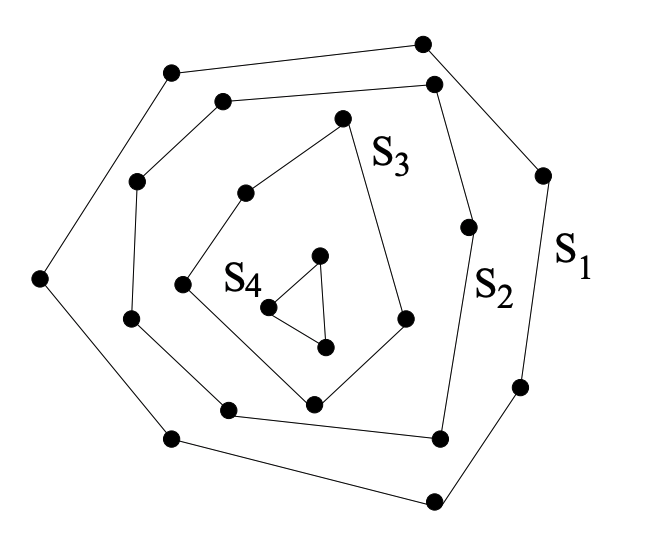
\includegraphics[width=0.25\textwidth]{onions}
    \caption{Problem 4: Onion peeling}
\end{figure}

\section*{Tips and Acknowledgements}

{\bf David Mount's tips for writing up homework solutions}: Whenever you are
asked to present an ``algorithm,'' you should present three things: the
algorithm, an informal proof of its correctness, and a derivation of its
running time.  Remember that your description is intended to be read by a
human, not a compiler, so conciseness and clarity are preferred over technical
details.  Unless otherwise stated, you may use any results from class, or
results from any standard textbook on algorithms and data structures. Also, you
may use results from geometry that: (1) have been mentioned in class, (2) would
be known to someone who knows basic geometry or linear algebra, or (3) is
intuitively obvious. If you are unsure, please feel free to check with me.

Giving careful and rigorous proofs can be quite cumbersome in geometry, and so
you are encouraged to use intuition and give illustrations whenever appropriate.
Beware, however, that a poorly drawn figure can make certain erroneous
hypotheses appear to be ``obviously correct.''

Throughout the semester, unless otherwise stated, you may assume that input
objects are in general position. For example, you may assume that no two points
have the same x-coordinate, no three points are collinear, no four points are
cocircular. Also, unless otherwise stated, you may assume that any geometric
primitive involving a constant number of objects each of constant complexity can
be computed in O(1) time

{\bf Acknowledgements:} Homework problems adapted from assignments of David
Mount and Carola Wenk.

\end{document}
